\documentclass{standalone}
  \usepackage{tikz}
  \usetikzlibrary{arrows.meta, automata, bending, positioning, shapes.misc}
  \tikzstyle{automaton}=[shorten >=1pt, >={Stealth[bend,round]}, initial text=]
  \tikzstyle{accepting}=[double]

\begin{document}
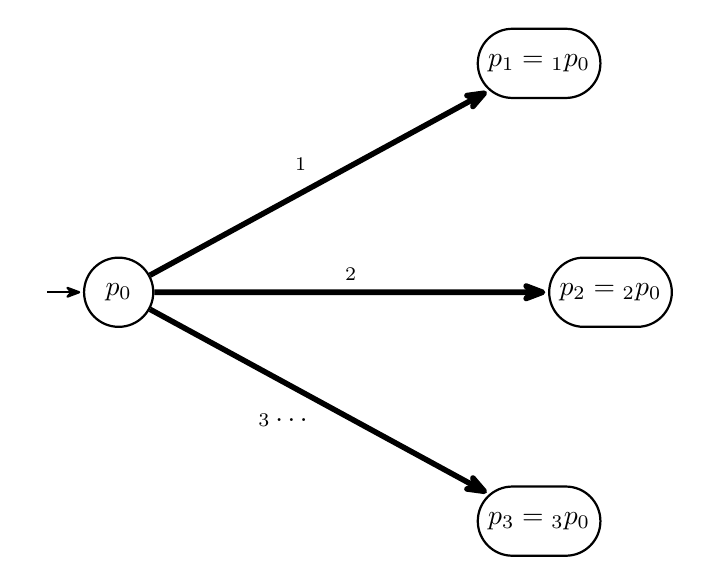
\begin{tikzpicture}[automaton, auto, thick]
  \node[state,initial,rounded rectangle] (0) {$p_0$};
  \node[state,rounded rectangle] (1) [above right=20mm and 50mm of 0] {$p_1 = \deriv{\typevar_1}{p_0}$};
  \node[state,rounded rectangle] (2) [right=50mm of 0] {$p_2 = \deriv{\typevar_2}{p_0}$};
  \node[state,rounded rectangle] (3) [below right=20mm and 50mm of 0] {$p_3 = \deriv{\typevar_3}{p_0}$};

  \path[->] (0) edge[line width=2pt] node {$\typevar_1$} (1);
  \path[->] (0) edge[line width=2pt] node {$\typevar_2$} (2);
  \path[->] (0) edge[swap,line width=2pt]  node[pos=.5] {$\typevar_3 \ldots$} (3);
\end{tikzpicture}
\end{document}
